%% LaTeX2e class for student theses
%% sections/content.tex
%% 
%% Karlsruhe Institute of Technology
%% Institute for Program Structures and Data Organization
%% Chair for Software Design and Quality (SDQ)
%%
%% Dr.-Ing. Erik Burger
%% burger@kit.edu
%%
%% Version 1.1, 2014-11-21

%To be able to reference labels in other file
\externaldocument{introduction}
\externaldocument{appendix}

%%%%%%%%%%%%%%%%%%%%%%%%%%%%%%%%%%%%%%%%%%%%%%%%%%%%%%%%%%%%%%%%%%%%%
%--WATERTANK--%
%%%%%%%%%%%%%%%%%%%%%%%%%%%%%%%%%%%%%%%%%%%%%%%%%%%%%%%%%%%%%%%%%%%%%
\chapter{Motivating Example: Refinement of CPS ``Water tank''}
\label{ch:Watertank}

To better understand the process of refinement of a CPS we take an example from the \keym~tutorial~\cite{keymaera}, a Water tank (See Fig.~\ref{fig:watertank}) whose water level is adjusted automatically to stay at a certain level, and refine its hybrid model to gain an implementation. Our goal therefore is finding a suitable and verified implementation from the hybrid model with all necessary proof steps. To accomplish this, we have to adjust and verify the hybrid model, code and verify a concrete implementation and finally verify the ``glue'' in between the discrete and continuous world we come up with as our last proof steep. 

\begin{figure}[h!]
	\setcounter{figure}{0}
	\centering
	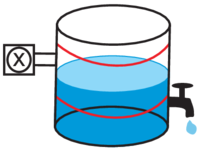
\includegraphics[width=0.6\textwidth]{images/watertank}
	\caption{Picture of possible Water tank configuration: Water tank that can get drained at all times and has a valve controlled by a control program~\cite{keymaeraGuide}.}
	\label{fig:watertank}
\end{figure}

\section{Detailing the Water tank CPS}
\label{sec:watertank:detail}

The ``control'' part of this hybrid system is the valve, it can either drain the water tank with a rate of \(-2\) or it can fill the tank further with a rate of \(1\). The goal of the entire system then is, to keep the water level \(y\) of the tank between \(1\) and \(12\). Normally this is proven by \keym~ without actually implementing a control program. To be able to we first took a look at the hybrid model of the water tank. It is provided both in the form of a hybrid automaton (See Fig.~\ref{fig:watertank_ha}) and a hybrid program (See Sec.~\ref{sec:watertank_hp}). In the hybrid automaton, the system starts in the ``fill'' state, where water is constantly flowing into the tank with the rate of \(y^{\prime} = 1\), while the clock is counting by \(x^{\prime}=1\) per tick. Once the water level reaches a certain level \(y=10\) the clock is reset to \(x:=0\) and the state changes from ``fill'' to ``stop'', where the water level is still raising for 2 ticks since the valve can not change in instant time. Once those 2 ticks pass \(x=2\) the water tank switches its state again to ``drain'' in which water flows out of the tank at the rate of 2 per clock tick, before it changes again to ``start'' the filling of the tank again once the water level hits \(y=5\).
\begin{figure}
	\centering
	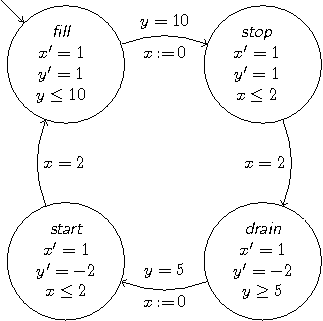
\includegraphics[width=0.6\textwidth]{images/watertank_ha}
	\caption{The Water tank CPS expressed as a hybrid automaton~\cite{keymaeraGuide}.}
	\label{fig:watertank_ha}
\end{figure}

\subsection{The original Hybrid Program}
\label{sec:watertank:hp}

The hybrid program (see App.~\ref{app:sec:pdfs} for HP expressed in ASCII) has three variables (water level y, time x and state st all as Real numbers) defined as:
\(\mathbb{R}~y, x, st;\) in the \(\\ProgramVariables\) section. Then the complete program notation with a preceding initialization of values and state.
\begin{flalign*}
		[ x:=0,y:=1, st:=0]& ((st = 0) \implies \\
			\quad& [ (?(st=0); \\
			\quad&\quad\quad(?(y=10); x:=0; st:=1) \\
			\quad&\quad\quad\cup (?(y<10 \vee y >10); x^{\prime}=1 \wedge y^{\prime}=1 \wedge y\leq10)) \\
			\quad&\cup (?(st=1); \\
			\quad&\quad\quad(?(x=2); st:=2) \\
			\quad&\quad\quad\cup(?(x<2\vee x>2);x^{\prime}=1, y^{\prime}=1 \wedge x\leq2)) \\
			\quad&\cup(?(st=2); \\
			\quad&\quad\quad(?(y=5);x:=0;st:=3) \\
			\quad&\quad\quad\cup(y>5\vee y<5); x^{\prime}=1,y^{\prime}=-2 \wedge y\geq5)) \\
			\quad&\cup(?(st=3); \\
			\quad&\quad\quad(?(x=2);st:=0) \\
			\quad&\quad\quad\cup[(?(x>2\vee x<2);x^{\prime}=1,y^{\prime}=-2 \wedge x\leq2)) \\
			\quad&](y\geq1\wedge y\leq12))		
\end{flalign*}


\section{The ``Hook'': Concrete Control Value Assignment}
\label{sec:Watertank:ControlValue}

In order to be able to apply Eq.~\ref{eq:Main:LogicRefinement} to this concrete example, we first found a spot in which a (or multiple) concrete control value is actually assigned. We call this assignment the \textit{hook} as the actual implementation will ``hook'' into our hybrid model at this exact point. The Hybrid Automaton describing the Water tank (See Fig.~\ref{fig:watertank_ha}), required changing to be able to find our actual ``hook''. In the original model, a control value is never explicitly assigned, rather does the valve change its state non-deterministically, making a deterministic control program implementation impossible, as the program can not act in a non-deterministic manner and would not fit in the model of the CPS. A version of the hybrid automaton with the hook marked in red can be found at App.~\ref{fig:ex_control}. Our remodeled system features a clear ticked hook that is called upon at deterministic times (See Sec.~\ref{sec:watertank_hp_ref}).

\subsection{Remodeled Hybrid Program}
\label{sec:watertank_hp_ref}
The remodeled hybrid program(see App.~\ref{app:sec:pdfs} for HP expressed in ASCII) has 5 variables and a constant: tick defined in the \(\\functions\) clause as being \(\in \mathbb{R}\), and water level y, time x, new valve value new and valve value from a tick ago valve which are defined in the \(\\programVariables\) clause as being \(\in \mathbb{R}\).
\begin{flalign*}
		tick > 2 &\implies \\
			&[ x:=tick,y:=1, valve:=1; \\
			\quad& (?(x=tick); new:=*; x:=0); \\
			\quad&\quad(?(y+2*valve+tick*new\geq1\wedge y+2*valve+tick*new \leq 12 \wedge{} \\
			\quad&\quad(new=1\vee new=2)); \\ 
			\quad&\quad\quad((?(new\neq valve); x^{\prime}=1, y^{\prime}=valve \wedge x \leq 2); \\
			\quad&\quad\quad\quad(\textrm{if } (x=2) \\
			\quad&\quad\quad\quad \textrm{then }valve:=new; x^{\prime} = 1, y^{\prime} = valve \wedge x \leq tick~\textrm{fi}) \\
			\quad&\quad\quad(?(\neg(new\neq valve)); x^{\prime}=1,y^{\prime}=valve\wedge x \leq tick)))] \\
			&(y \geq 1 \wedge y \leq 12)	
\end{flalign*}


We kept the model mostly equivalent to the original, preserving the two clock ticks of time needed for the valve to change its state from drain to fill and vice-versa. This presented a challenge, when thinking of possible implementations, as the program hook could be called again before the valve would have actually changed its state. To simplify this problem, we only model cases in which the actual program tick (so the time between two hook calls)  is greater than two clock ticks (however long they may be). This means, that the valve or control program does not have to have a (possibly infinite) list of the last control values assigned, which could be the case if the program was called more frequently than the valve is able to change states.

\section{Implementation Safety Condition}
\label{sec:Watertank:SafetyCond}

Next we devised a postcondition for the implementation hook, which would then serve as the abstraction of the Java control program. This means, that the program would be built accordingly, so that it could be verified against this postcondition. It therefore also served as a form of specification for us when devising the implementation. The original postcondition we devised:

\begin{equation}
	\centering
	\begin{split}
		\psi \equiv (y + 2* valve + tick -2 * new  \geq 1 \wedge \\ 2 * valve * (tick - 2) * new \leq 12 \wedge \\  y + 2* valve \geq 1 \wedge  y + 2 * valve \leq 12) 
	\end{split}
\label{eq:postCondOrig}
\end{equation}

During verification of the new hybrid program, \keym would not verify the program with this postcondition. This means, that even in such a simple CPS as this water tank control system, finding the hook postcondition was non-trivial and only with the help of \keym's counterexample-search did we manage to find the correct postcondition (See Eq.~\ref{eq:postCondOrigCorrect}). 

\begin{equation}
	\centering
	\begin{split}
		\psi \equiv (y + 2 * valve + tick * new \geq 1 \wedge\\ y + 2 * valve + tick * new \leq 12 \wedge \\(new = 1  \vee new = -2))
	\end{split}
	\label{eq:postCondOrigCorrect}
\end{equation}

\keym~ verified our new hybrid program fully automatically.

\section{The (simple) Java Control Program}
\label{sec:Watertank:Java}

After completing verification of our hybrid model with \keym, we proceeded to implement a (simple) control program for the Water tank. Finding a suitable implementation proved difficult, as a parallel implementation (Both the control system and the differential equations working in parallel, modifying the water level) seemed more intuitive. This would defeat the purpose of actually finding a suitable hook and was more based on our understanding of the original hybrid model and not our version including the hook.

Using our understanding of a singular hook of the control system into the water tank as well as the hook postcondition from the previous section as our specification for the actual control method, that would return the control value to the water tank's valve, we then managed to implement a suitable discrete control method (See Lst.~\ref{lst:source:controlMethod}). As can be seen, the control method is relatively simply and only assigns the best/worst case scenario values. For the entire control class see App.~\ref{app:lst:watertankContr}.

\definecolor{darkgreen}{rgb}{0.0, 0.2, 0.13}
\lstset{language=Java,captionpos=b,tabsize=3,frame=lines,keywordstyle=\color{blue},commentstyle=\color{darkgreen},stringstyle=\color{red},numbers=left,numberstyle=\tiny,numbersep=5pt,breaklines=true,showstringspaces=false,basicstyle=\footnotesize,emph={label}}
\begin{lstlisting}[label=lst:source:controlMethod]
public int getControlValue (int y, int old) {
		//Waterlevel in two time units
		int inTwo = y + 2 * old;
		//If we are raising level, keep raising if possible without hitting max_level before next tick
		if (old == 10) {
			if (inTwo + tick * 1 <= 116) {
				return 10;
			}
			else {
					return -20;
			}
		}
		//ELSE if we are currently lowering level, keep lowering if we can lower further without hitting min_level b4 next tick
		else {
			if (old == -20) {
				if (inTwo - tick * 2 >= 12) {
					return -20;
				}
				else {
						return 10;
				
				}
		
			}
		}
		//Only returned if old != 10 && old != -20, unreachable.
		return 0;
}
}
\end{lstlisting}

The control method consists only of simple if-else-statements and just assigns the best-case (keep raising level if we were raising, keep lowering if we are lowering as long as postcondition is still valid) value to the valve. We translated the hook postcondition (See  Eq.~\ref{eq:postCondOrig}) into, what we thought to be at the time, a suitable JDL postcondition statement for verification with \key~(See List.~\ref{lst:JDL}). In the next section we will explain why this postcondition would not work for our complete proof. \key~verified our program fully automatically, aside from the fact, that the \(tick>2\) precondition added too much computational complexity, so we let \key~prove the property with the more concrete \(tick==30; \textrm{ or }tick==31;\dots\) assignments. 

For testing purposes, we also implemented a complete simulator of the Water tank CPS (See App.~\ref{app:lst:watertankSim}).

\begin{lstlisting}[label=lst:JDL]
	/*@ public normal_behavior 
	  @ requires tick == 30 && y >= 10 && y <= 120 && y + 2 * old <= 120 && y + 2 * old >= 10 && (old == 10 || old == -20);
	  @ ensures \result * (tick / 10) + y + 2 * old  >= 12 & \result * (tick / 10) + y + 2 * old <= 116 && (\result == 10 || \result == -20); 
	  @*/
\end{lstlisting} 

\section{Glue between Java and Hybrid Model}
\label{sec:Watertank:Glue}

As real values (used in the hybrid model) and discrete values (used in our Java implementation) are fundamentally different, a certain transformation has to occur.  In the Water tank example, this means, that the water level as well as the last valve-value (be it fill or drain), which are passed to the control method, have to be converted into one direction by the glue. 

Also, the result of the computation in the method (so the new valve value) has to be converted in the other direction. In general the glue is not necessarily a bijective function, as some values will not exist in both worlds, making it a relation. For the Water tank, fortunately, this problem doe not exist, so finding a function translating the water level and valve values into each other instead of a relation simplifies the problem.

Finding the glue between the real parts of the hybrid system and our Java control program still proved difficult though.

As we went along, we figured out how a general glue proof should look (See Fig.~\ref{eq:glueGeneral}). Here \(x\) are the discrete values in our control program, \(y\) are the real world values, \(\psi\) is the postcondition of the control program expressed using discrete values and \(\phi\) is the actual safety condition we want to show for the entire hybrid system.

\begin{equation}
	\centering
	\begin{split}
		\forall~x \in (Discrete World)~\forall~y \in (Real World):(x,y) \in \textit{glue} \implies (\psi(x) \implies \phi(y))
	\end{split}
	\label{eq:glueGeneral}
\end{equation}

Following this basic guideline, we were able to find a suitable glue relation (or in our case total relation) for this CPS. We found the following as the glue-relation:

\begin{equation}
	\begin{split}
		\forall~y \in \mathbb{R}~. \forall~y_j \in \mathbb{Z}. \forall~valve \in \mathbb{R}. \forall~tick \in \mathbb{R}&. \forall~tick_j \in \mathbb{Z} . \forall~new \in \mathbb{Z}. \forall~result \in \mathbb{R}~: \\  y_j = \textrm{floor}(10 * y)~\wedge&~ old_j = \textrm{floor}(10*valve) \wedge tick_j = \textrm{floor}(10*tick)~\wedge \\ result = 10 * new~\wedge&~ y \geq 1~\wedge~y \leq 12~\wedge  (valve = 1 ~\vee~valve = -2)~\wedge \\&tick > 2 
	\end{split}
	\label{eq:glueWatertank}
\end{equation}

Whereby \(\psi(x)\) is equivalent to:
\begin{equation}
	\begin{split}
		result * tick_j/10 + y_j + 2 * old_j \leq 116~\wedge&~result * tick_j/10 + y_j + 2 * old_j \geq 12~\wedge \\ (result = 10~\vee&~result = -20)
	\end{split}
	\label{eq:psiWatertank}
\end{equation}

And \(\phi(y)\) is equivalent to:

\begin{equation}
	\begin{split}
		 y + 2 * valve + tick * new \geq 1~\wedge&~y + 2 * valve + tick * new \leq 12~\wedge \\ (new = 1~\vee&~new = -2)
	\end{split}
	\label{eq:phiWatertank}
\end{equation}

As can be seen, the \(\psi(x)\) that we found for the glue is not equal to the original trivial postcondition for our Java program (See List.~\ref{lst:JDL}). This can be explained by the floor functions that has to be used for translation from the \(\mathbb{R}\) into \(\mathbb{Z}\) world. Due to the usage of the floor function, we only can approximate the original value in the discrete world, and therefore these approximation errors have to be accounted for in \(\psi\). Again the fact that we only found this error in our original postcondition devised for the Java program, proves the non-triviality of the process even in seemingly simple examples as this water tank. The glue in ASCII notation can be found in App. Sec.~\ref{app:sec:pdfs}.

\section{Verification based on \keym}
\label{sec:Watertank:Verification}

Verification of the glue proved difficult since \keym, or specifically Mathematica (cf.~\cite{mathematica}) (\keym~backend algebraic solver), has problems with the translation of uninterpreted functions. Therefore we found an abstraction of the floor function using inequalities to approximate it:

\begin{align*}
		\forall~x \in \mathbb{R}. \forall~c \in \mathbb{R}. floor(x) = c \implies x-1 < c \wedge c \leq x \wedge( x>0\implies c>0)
	\label{eq:approxF}
\end{align*}
Also, since \keym~does not deal with numbers outside of the reals, we generalized the preconditions for every variable to be in the reals. This obviously only strengthens the proof and therefore does not change the correctness.

This still lead to problems when using the automatic proof-mechanism, so we had to add a full new taclet fdef to the definition file to be able to use the automatic prover (See App..~\ref{app:lst:ruleF}).

The proof runs fully automatically with our own defined taclet.

%%%%%%%%%%%%%%%%%%%%%%%%%%%%%%%%%%%%%%%%%%%%%%%%%%%%%%%%%%%%%%%%%%%%%
%--PROCESS--%
%%%%%%%%%%%%%%%%%%%%%%%%%%%%%%%%%%%%%%%%%%%%%%%%%%%%%%%%%%%%%%%%%%%%%
\chapter{Formalized approach of refining hybrid models into implementation}
\label{ch:Process}

What the Water tank example shows is the non-triviality of refining the hybrid model into an implementation and of the verification of all necessary parts. Overall it is obvious, that a formalized approach to the general problem presented in chapter~\ref{ch:Introduction} is necessary. In this chapter we present a possible formalized approach to the problem, that we deemed feasible.
\\


To aid readability we will now give an overview of the process without explanation, then detail each step in the following sections. 

\begin{enumerate}
	\item Modeling CPS as Hybrid System that includes concrete hook.
	\item Finding the necessary safety condition of the control value for verification with \keym.
	\item Implementing control program according to (preliminary) safety condition and Verification by \key.		
	\item Finding the correct ``glue'' between hybrid model and control program and its verification by \keym.
	\item Result validation: Does our implementation still match the correct safety condition after verifying the glue?
\end{enumerate}

Overall for verification of our resulting implementation three proof obligations exist:
\begin{enumerate}[label=\roman*]
	\item Proving correctness of our hybrid model that includes a hook and the hook postcondition with \keym.
	\item Proving correctness of our implementation according to the (preliminary) safety condition and verifying it against it using \key.
	\item Proving correctness of our glue using \keym.
\end{enumerate} 

With correct verification of all three parts, we can deduce that Eq.~\ref{eq:Main:LogicRefinement} has been fulfilled and our goal has been reached of creating a verified concrete implementation for a CPS.

In a more formalized manner this could be expressed as in Eq.~\ref{eq:form:goal}, whereby HP is the Hybrid Program representation of the CPS, \(\psi(x)\) refers to the hook postcondition, \(\alpha\) is the safety property of the entire system that has to be shown, Java just refers to the concrete Java implementation, \(\phi(y)\) is the Java World postcondition (often differes from \(\psi(x)\) due to rounding/flooring) and \(x:=Java\) refers to the hook that is replaced by the actual implementation.
\begin{equation}
	\begin{split}
		HP[\dots x:=*; ?\psi(x) \dots](\alpha) {}\wedge{}& \\ Java[\dots y:=newY \dots](\phi(y)) \wedge{}& \\ glue(x,y) \implies{}& HP[\dots x:= Java; ?\psi(x)\dots](\alpha)
	\end{split}
\label{eq:form:goal}
\end{equation}

\section{Modeling Hybrid System with Implementation Hook}
\label{sec:Process:Hook}
Most CPS we took a look at (See \cite{keymaera} Tutorial, \cite[p.~5, p.~11]{platzer2010b} \dots) as examples, did not have a concrete spot in which a control program could ``hook'' in easily. This means, that the first step in our refinement process has to be finding a suitable hook for the control program, referring to one or more non-deterministic assignments of a/multiple control values. Mostly for already existing hybrid systems, as was the case in Sec.~\ref{sec:Watertank:ControlValue}, a complete changing of the model is necessary. When creating a new model, one should try to find a suitable spot for a non-deterministic control value assignment. As a discrete deterministic control program can only be enacted at certain times, a model of a form of tick has to be found, as to make an actual implementation feasible. Mostly this will result in an extra condition for the entire hybrid program, as we only want the program to work if the differential equations run till the discrete tick (See Sec.~\ref{sec:watertank_hp_ref}).

To prevent issues in later verification of the model, a hybrid program and not a hybrid automaton representation of the model should be chosen, as an automaton cannot be verified using the compositional verification approach of \keym(cf.~\cite[ch.~1.1.4]{platzer2010b}). Since the modeling of the system can often be incorrect and a formal way to verify if the model correctly models all necessities does not exist, great care should be enacted during modeling or remodeling of the CPS.

\section{Devising Control Value Safety Postcondition}
\label{sec:Process:SafetyCond}

After finding a suitable hook spot in our program we have to the analyze the hook for a safety condition. If we think back to the water tank example (See Sec.~\ref{sec:Watertank:SafetyCond}), this was non-trivial as the first postcondition we came up with through logic deduction proved to be incorrect. When thinking of possible conditions we often found we overlooked the tick when considering different postconditions. Obviously, more than one valid postcondition exists, as the constraints imposed on the implementation can get arbitrarily strong and we're not restricting the actual behavior of the physical part of the CPS, it only restricts the system to the cases we want to actually consider in our analysis.

One should try and find the most general postcondition \(\psi\) for which the safety condition still holds, as this makes it easier to code the actual implementation with less constraints. Of course, if the model's proof works without any postcondition, this means that the program could also just assign random values making the implementation and glue trivial or non-existent. With correct modeling and sufficiently complex hybrid system (which even the relatively easy water tank had) this should never occur though.

The entire hybrid model with the hook safety postcondition should then be verified by \keym. In certain cases, abstractions or simplifications of the original problem on hand have to be inserted (e.g. in our water tank case the precondition \(tick>2\)), as to not put \keym's automatic verification mechanism under too much strain.

\section{Implementation according to Postcondition and its Verification}
\label{sec:Process:Implementation}

Implementation of the program can theoretically be done in any preferred language, for usage with \key~as the automatic prover, Java or other C-like languages are preferred. The implementation is free from any constraints asides from the postcondition that was devised previously, and from the constraints required by \key~(or the alternative automatic verification program in use) itself (No threading etc. for \key). Since the postcondition is in the hybrid model and therefore written in the form of real variables and values, one has to already think of a form of the glue that will be formally devised in the next step, as to find a suitable translation of the postcondition expressed with real values into JDL. The postcondition in JML will most likely only be a preliminary condition, as it is possible (and rather likely due to rounding and/or flooring) (as in Sec.~\ref{sec:Watertank:Glue}) that the formal glue will show that the original postcondition does not work when then replacing the hook with the implementation. 

While an automatic generation of a correct implementation according to the predefined safety condition would certainly be possible, the automatic generation brings with itself a few issues, namely and mostly that an automatically generated implementation is bound to be less real-world applicable. As for example the easiest implementation for many of these CPS control programs could just return the safest possibility (e.g, not changing the water level at all, or braking at the maximum braking speed). Often real-world applicable implementations require more functionality, which we try and implement and show our approach is sound for more complicated less trivial implementations as well.

The implementation with its postcondition expressed in JDL then has to be verified by \key~before continuing with the glue. 

\section{Glue between Hybrid Model and Implementation and its Verification}
\label{sec:Process:Glue}

As both our model and implementation are now verified, the actual glue between the implementation and the model has to be devised. In the previous Chapter we came up with a general definition of what the glue relation provides:

\begin{equation}
	\centering
	\begin{split}
		\forall~x \in (Discrete World)~\forall~y \in (Real World):(x,y) \in \textit{glue} \implies (\psi(x) \implies \phi(y))
	\end{split}
	\tag{\ref{eq:glueGeneral}}
\end{equation}

Coming up with the glue is the hardest part of the entire process, and took multiple iterations before a correct and verified glue was found for our studied examples. Most of the time the glue will probably incorporate some form of rounding/flooring mechanism, as we have to translate real values into discrete ones. This makes the entire proof hard to fully understand for humans without lots of complex mathematical computations.

We used a form of logical deduction to come up with the correct quantifiers for the glue proof (so the \(\forall\) in Eq.~\ref{eq:glueGeneral}), since if there only \(\exists\) a Java-equivalent for a certain real-world variable, issues arise when analyzing the glue in the other direction (discrete -> real). Verification of the glue should then happen using \keym, which means formulation of the glue should already be in the required syntax.

Overall this means, that for the discrete-world postcondition \(\psi\) that was proven by \key~, the real-world postcondition \(\phi\) found in Sect.~\ref{sec:Process:SafetyCond}, and the glue that we devise which is verified by \keym, we reach the goal we set out for (See Ref. ~\ref{eq:Main:LogicRefinement}).

\section{Validating Verification results against Implementation}
\label{sec:Process:Eval}

As we realized in our Water tank example (See Sec.~\ref{sec:Watertank:Glue}), with verification of our glue some changes might have to be made to the implementation and its postcondition. To complete the process of refinement we have to change the implementation and JDL condition and verify it again with \key. At last we then make sure all our decisions made were actually valid and correct when taking a look back at the entire picture as outlined in Ref.~\ref{eq:Main:LogicRefinement}.


%%%%%%%%%%%%%%%%%%%%%%%%%%%%%%%%%%%%%%%%%%%%%%%%%%%%%%%%%%%%%%%%%%%%%
%--TRAFFIC CONTROL--%
%%%%%%%%%%%%%%%%%%%%%%%%%%%%%%%%%%%%%%%%%%%%%%%%%%%%%%%%%%%%%%%%%%%%%
\chapter{Evaluation using Example CPS: ``Traffic Speed Control''}
\label{ch:Traffic}

After formalizing our approach used in the opening water tank example, we now want to prove its feasibility on a new and fresh example. The following example is taken from~\cite{TrafficControl} and describes a two-part control system responsible for a one-way linear freeway on which speed limits are set randomly by one part of the control system and the single moving car's acceleration is set by the car control's part of the program. The goal for the system is to never let the car break the speed limit at any point. This means the two control systems have to communicate, which also has to be represented in the hybrid system.  

\begin{figure}[h!]
	\centering
	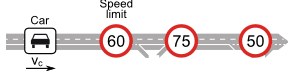
\includegraphics[width=0.6\textwidth]{images/trafficControl}
	\caption{The set-up of this CPS~\cite{keymaera}.}
	\label{fig:trafficControl}
\end{figure}

To show feasibility of our newly found approach, we now follow the process outline from the previous chapter. The first step is remodeling the CPS as to include a hook and a suitable safety condition and verifying it, followed by implementation and verification of the entire system. 

\section{Remodeling with Hook}
\label{sec:traffic:hook}

When taking a look at the original hybrid program notation of the traffic control CPS (See Eq.~\ref{eq:traffic:orig}), one can see the complexity of this problem. Here, \(t\) is the time, \(x_1\)\ is the position of the car, \(x_{sl}\) is the position of the next speed limit, \(v_1\) is the speed of the car, \(v_{sl}\) is the speed limit, \(A\) is the maximum acceleration, \(B\) is the maximum braking power and \(ep\) is the maximum communication time between the car and speed limit controller. This hybrid program notation already obviously brings a high level of complexity and is hard to understand, so we decided to simplify the problem during remodeling. 

\subsection{Remodeled Hybrid Program}
\label{subsec:traffic:remodel}
To simplify the problem at hand, we first removed the communication time ep, by arguing, that it can be 0 without affecting the correctness of the model, but for our purposes we use ep as the length of the tick, as this is the time in which we cannot exert control over the system, so for us the time we cannot exert control is only tick and the communication time equals 0. To introduce the tick in the hybrid program we use the same trick as in the water tank example by only ``executing'' the differential equations when the tick was reached and forcing them to run the full duration until the next tick every time. Also, for simplification we tick the speed limit control system synchronized to the car control system, as to remove complexity and make implementation easier. This seems plausible in reality and we forgo the need to model/implement the communication between both control programs. Our remodeled hybrid program can be seen in Eq.~\ref{eq:traffic:rem}. Here, the two hooks can be seen at \(a_1:=*;\) and \(x_{sl} :=*; v_{sl} := *;\) .

In our remodeled version, the car is controlled at an arbitrary time \(t~mod~ep\equiv0\), whose control program then ensures safety for the car until the next tick occurs and the program is enacted again, meaning if the car breaks at maximum braking speed\( B\) at the next tick it can still reach a safe position/speed. Then at the same time t the second hook for the speed limit control program is enacted, where another postcondition has to be checked as to make sure the new chosen speed limit is in a safe spot for the car.

\phantomsection
\label{eq:traffic:orig}
\begin{flalign*}
 v_1 \geq 0 \wedge{}& v_{sl} \geq 0 \wedge x_1 \leq x_{sl} \\
 {}\wedge{}&  2 * B (x_{sl} - x_1) \geq v_1^{2} - v_{sl}^{2} \\
 {}\wedge{}& A \geq 0 \\
 {}\wedge{}& B \geq 0 \\
 {}\wedge{}& ep \geq 0 \implies \\
			[& a_1 := -B \\
			\quad&\quad\quad \cup (?(x_{sl} \geq x_1 + (v_1^{2}-v_{sl}^{2}) / (2*B) + (A / B + 1) * (A / 2 * ep^2 + ep * v_1)) ; \\
			\quad&\quad\quad\quad a_1:= *; \\
			\quad&\quad\quad\quad?(-B \leq a_1 \wedge a_1 \leq A)) \\
			\quad&\quad\quad\cup (?(x_1 \geq x_{sl}); \\
			\quad&\quad\quad\quad a_1 := *; \\
			\quad&\quad\quad\quad ?(-B \leq a_1 \wedge a_1 \leq A \wedge a_1 \leq (v_1- v_{sl}) / ep)); \\
			\quad&\quad\quad (x_{sl} := x_{sl}; \\
			\quad&\quad\quad\quad v_{sl} := v_{sl}) \\
			\quad&\quad\quad \cup (x_{sl} := *; \\
			\quad&\quad\quad\quad v_{sl} := *; \\
			\quad&\quad\quad\quad ?(v_{sl} \geq 0 \wedge x_{sl} \geq x_1 + (v_1^{2} - v_{sl} ^{2}) / (2*B) + (A/B + 1) *  (A / 2 * ep^2 + ep * v_1))); \\
			\quad&\quad\quad t:=0; \\
			\quad&\quad\quad \{ a_1^{\prime} = v_1, v_1^{\prime} = a_1, \\
			\quad&\quad\quad t^{\prime} = 1, v_1 \geq 0 , t \leq ep\})* \\
			 ]& (x_1 \geq x_{sl} \implies v_1 \leq v_{sl}) 
\end{flalign*}
\phantomsection
\label{eq:traffic:rem}
\begin{flalign*}
 v_1 \geq 0 \wedge{}& v_{sl} \geq 0 \wedge x_1 \leq x_{sl} \\
 {}\wedge{}&  2 * B (x_{sl} - x_1) \geq v_1^{2} - v_{sl}^{2} \\
 {}\wedge{}& A \geq 0 \\
 {}\wedge{}& B \geq 0 \\ 
 {}\wedge{}& ep \geq 0 \implies \\
			[& ( \\
			\quad&\quad\quad?(t=ep); \\
			\quad&\quad\quad(a_1 := *); \\
			\quad&\quad\quad?(-B \leq a_1 \wedge a_1 \leq A \wedge (x_1 \geq x_{sl} \implies (a_1 \leq (vsl - v1) / ep)) \\
			\quad&\quad\quad{}\wedge (x_1 < x_{sl} \implies (x_{sl} \geq x_1 + (v_1^2 - v_{sl}^2) / (2 * B) + (A / B + 1) * (A / 2 * ep^2 + ep * v_1)))); \\
			\quad&\quad\quad x_{sl} := *; v_{sl} := *; \\
			\quad&\quad\quad\quad ?(v_{sl} \geq 0 \wedge v_{sl} < v_1 \implies{}  \\
			\quad&\quad\quad\quad x_{sl} \geq x_1 + (v_1^{2} - v_{sl} ^{2}) / (2*B) + (A/B + 1) *  (A / 2 * ep^2 + ep * v_1)) \\
			\quad&\quad\quad\quad {}\wedge  v_{sl} \geq v_1 \implies a_1 \leq (v_{sl} - v_1) / ep)); \\
			\quad&\quad\quad t:=0; \\
			\quad&\quad\quad \{ x_1^{\prime} = v_1, v_1^{\prime} = a_1, \\
			\quad&\quad\quad t^{\prime} = 1, v_1 \geq 0 , t \leq ep\})* \\
			 ]& (x_1 \geq x_{sl} \implies v_1 \leq v_{sl})
\end{flalign*}

\section{Safety Hook Postconditions}
\label{sec:traffic:postcondition}

Following our process outline, the next step is to find a suitable safety postcondition for the two hooks. Using logic deduction we came up with two suitable safety postconditions (See Eq.~\ref{eq:traffic:post1},~\ref{eq:traffic:post2}), as \keym~then automatically verifies the entire hybrid model. In the first postcondition, meant for the car control program, the chosen acceleration for the car has to be in between the minimum and maximum acceleration and the acceleration has to be chosen in such a way, that both cases are safe: 1) the car is currently before the speed limit, we accelerate in a way so that we can still break with the maximum braking speed at the next tick and stay under the limit or to the right of the speed limit. 2) If the car is already in the speed limited zone we accelerate in such a way that we don't reach a speed higher than the speed limit until the next tick. The second postcondition, responsible for the speed limit chooser program, has to make sure that the new speed limit is bigger than 0 (so as to make it possible for the car to even keep the speed limit), and that the speed limit is chosen in such a way that the car can still break with the maximum brake speed and be safe, in both cases (left of the speed limit/right of the speed limit).

\begin{equation}
\begin{split}
	\phi_1 \equiv&-B \leq a_1 \wedge a_1 \leq A \wedge (x_1 \geq x_{sl} \implies (a_1 \leq (vsl - v1) / ep)) \\
	 {}\wedge{}& (x_1 < x_{sl} \implies (x_{sl} \geq x_1 + (v_1^2 - v_{sl}^2) / (2 * B) + (A / B + 1) * (A / 2 * ep^2 + ep * v_1)))
	\end{split}
	\label{eq:traffic:post1}
\end{equation}
	
	
\begin{equation}
\begin{split}
	\phi_2\equiv (v_{sl} \geq 0 \wedge v_{sl} < v_1 \implies{}   x_{sl} \geq x_1 + (v_1^{2} - v_{sl} ^{2}) / (2*B) + (A/B + 1) *  (A / 2 * ep^2 + ep * v_1)) \\
	{}\wedge  v_{sl} \geq v_1 \implies a_1 \leq (v_{sl} - v_1) / ep))
\end{split}
	\label{eq:traffic:post2}
\end{equation}

\section{Implementation according to postconditions}
\label{sec:traffic:impl}

For the implementation of the two control programs we chose to use a conservative, easier to understand approach, as to make automatic verification using \key~possible. As there are two control programs/methods in use here, we just established the necessary ``communication'' between both through our third Simulator class (See App.~\ref{app:sec:TrafficSim}). 

\subsection{The Car Control Program}
\label{subsec:traffic:car}
For the car control program (See List.~\ref{lst:carControl}), one can see, that we only change the acceleration value by one if it fulfills the safety condition and break the maximum amount if not. This means, that more often than not we will be breaking at full speed,  and this control program could be improved greatly in future work. We over approximate the conditions, as to fulfill our glue proof obligations as presented in Sec.~\ref{sec:traffic:glue}.

\begin{lstlisting}[label=lst:carControl]
public int control(int y, int v, int accel, int sl, int slPos) {
		if (y >= slPos - 1 && y < slPos + 1) {
			return MAXBREAK + 1;
		}
		if (y >= slPos - 1) {
			if ((accel+1)*TICK <= (sl-v) - 2 * TICK) {
				if (accel+2 <= MAXACCEL) {
					return accel+1;
				}
				
			}
			else {
				if((accel-1)*TICK <= (sl-v) - 2 * TICK) {
					if (accel-2 >= MAXBREAK) {
						return accel-1;
					}
			}
			}
		}
		if (y < slPos + 1) {
			if (slPos >= (y+1) + (v+1)*(v+1)  + ((accel+1)+1 +1) * ((accel+1 + 1) * TICK*TICK + TICK * (v+1))) {
				if (accel+2 <= MAXACCEL) {
					return accel+1;
				}
			}
			else {
				if (slPos >= (y+1) + (v+1)*(v+1)  + ((accel-1)+1 +1) * ((accel-1 + 1) * TICK*TICK + TICK * (v+1))) {
					if (accel-2 >= MAXBREAK) {
						return accel-1;
					}
				}
			}
		}
			return MAXBREAK + 1;
		
	}
\end{lstlisting}

In the contract we define for the car control program (See List.~\ref{lst:CondCar}),  one can see we had to explicitly list the value of the TICK and MAXBREAK/MAXACCEL as to make the automatic verification with the amount of computational complexity possible. We also had to give both the invariant as well as safety condition of the hybrid program as a precondition for the method, as we also did in our first water tank example (See List.~\ref{lst:JDL}), or in this case, an abstraction of the safety condition, namely that if we break at the MAXBREAK speed, we will be safe (or due to flooring at the MAXBREAK+1 speed), the first two preconditions can be seen as an invariant of the method, as we cannot control the acceleration level in our limit, if the acceleration level we get already violates this safety condition.
\begin{lstlisting}[label=lst:CondCar]
/*@ public normal_behavior
	  @ requires MAXBREAK <= accel - 1 && accel + 1 <= MAXACCEL && v >= 0 && sl >= 0 && TICK == 1 && MAXBREAK == -10 && MAXACCEL == 10 && ((!(y >= slPos - 1)) || ((MAXBREAK+2)*TICK <= ((sl - v) - 2 * TICK))) && ((!(y < slPos + 1)) || (slPos >= (y+1) + (v+1)*(v+1)  + (MAXBREAK + 2 + 1) * ((MAXBREAK + 2) * TICK*TICK + TICK * (v+1))));
	  @ ensures \result - 1 >= MAXBREAK && \result + 1 <= MAXACCEL  && ((!(y >= slPos - 1)) || (\result*TICK <= (sl - v) - 2 * TICK)) && ((!(y < slPos + 1)) || (slPos >= (y+1) + (v+1)*(v+1)  + (\result+ 1 + 1) * ((\result + 1) * TICK*TICK + TICK * (v+1))));
	 @*/
\end{lstlisting}

\subsection{The Speed Limit Control Program}
\label{subsec:traffic:speed}

List.~\ref{lst:programSpeed} shows the source code of the control method of our Speed Limit controller. The control method implements the two control values it has to assign by creating an array and returning the results in the array. The implementation proved interesting, as it has a certain freedom in choosing the next speed limit, as the control method could be trivial in case of just always returning the current speed limit and position, then the car would just continue with exactly it's current movement until it has to break and then come to a full stop. The control method tries to raise the current speed limit by one if we currently have a low speed limit set and lower it if we have a high speed limit set. We then assign the position of the speed limit as great enough to still be correct according to the set safety condition. We have to over approximate the safety conditions, because we have a rounding/flooring function from the glue (See sec.~\ref{sec:traffic:glue}). Again this control method errs on the side of caution and does not have a mathematically very interesting way to assign new values, something that could be improved upon in future work. The complete source code for the control class can be found in App.~\ref{app:lst:speed}.

\begin{lstlisting}[label=lst:programSpeed]
public int[] control(int y, int v, int accel, int sl, int slPos) {
		int[] result = new int[2];
		result[0] = sl;
		result[1] = slPos;
		if (sl<25) {
			if (sl+1 < v + 1 && sl+1 >= v - 1) {
				return result;
			}
			if (sl+1 < v + 1) {
				result[0]++;
				result[1] = y+1 + ((v+1)*(v+1)) + (MAXACCEL  + 2) * ((MAXACCEL+1) * TICK*TICK +  TICK * (v+1));
			}
			if (sl+1 >= v -1) {
				if (accel*TICK <= result[0]+1 - v - 2 * TICK) {
					result[0]++;
				}
			}
		}
		else {
			if (sl-1 < v + 1 && sl-1 >= v - 1) {
				return result;
			}
		if (result[0]-1 < v) {
			if (result[0]-1 >= 0) {
			result[0]--;
			
			result[1] = y+1 + (v+1)*(v+1) + (MAXACCEL  + 2) * ((MAXACCEL+1) * TICK*TICK +  TICK * (v+1));
			}
		}
		if (sl-1 >= v - 1) {
			if (accel*TICK <= ((result[0]-1 - v)-2*TICK) && result[0]-1 >= 0) {
				result[0]--;
			}
		}
	}
		return result;

	}
	}
\end{lstlisting}


In the contract we establish for the speed limit control method (See List.~\ref{lst:condSpeed}), \key~again only verified the method after we added explicit numbers for MAXBREAK, MAXACCEL and the TICK, but these can be replaced easily in the precondition and \key~still completes the verification.We had to add the postcondition from the car control program as well as the invariant/safety condition from the hybrid program as these are part of the entire system and have to hold true during the entire system's evolution.
\newpage
\begin{lstlisting}[label=lst:condSpeed]
/*@ public normal_behavior
	  @ requires MAXBREAK == -10 && MAXACCEL == 10 && TICK == 1 && v >= 0 && sl >= 0 && ((!(sl < v + 1)) || slPos  >= y+1+ (v+1)*(v+1) + (MAXACCEL + 1 + 1) * ((MAXACCEL+1) * TICK*TICK + TICK * (v+1))) && ((!(sl >= v - 1)) || accel*TICK <= ((sl - v) - 2 * TICK));
	  @ ensures \result[0] >= 0 && ((!(\result[0] < v + 1)) || \result[1]  >= y+1 + ((v+1)*(v+1)) + (MAXACCEL + 1 + 1) * ((MAXACCEL+1) * TICK*TICK + TICK * (v+1))) && ((!(\result[0] >= v - 1)) || accel*TICK <= ((\result[0] - v) - 2 * TICK));
	*/
\end{lstlisting}

\section{Glue between Java and Hybrid Program}
\label{sec:traffic:glue}

The glue for this CPS proved interesting, as for two hook postconditions we also had to devise two proof parts. Aside from this, the complexity of the involved proof parts meant, we had to split up each proof into smaller components as to be able to use \keym's automatic verification mechanism. For every glue part we again quantify all the variables as \(\forall~\mathbb{R}\) (See Eq.~\ref{eq:trafficQuant}). We also did not use the taclet we wrote for the water tank floor-function, rather putting in the abstraction of the flooring function into our preconditions explicitly to further reduce computational complexity for \keym.

\begin{equation}
	\begin{split}
	\forall~\mathbb{R}~x_1 .\forall~\mathbb{R}~v_1 .\forall~\mathbb{R}~a_1 .\forall~\mathbb{R}~v_{sl} .\forall~\mathbb{R}~x_{sl} .\forall~\mathbb{R}~B .\forall~\mathbb{R}~A . \forall~\mathbb{R}~ep . \\ \forall~\mathbb{R}~x_j .\forall~\mathbb{R}~v_j .\forall~\mathbb{R}~a_j .\forall~\mathbb{R}~sl .\forall~\mathbb{R}~slPos .\forall~\mathbb{R}~MAXBREAK .\forall~\mathbb{R}~MAXACCEL .\forall~\mathbb{R}~TICK .
	\end{split}
	\label{eq:trafficQuant}
\end{equation}

\subsection{Glue for the Car Control Program}
\label{subsec:traffic:carGlue}

For each proof part, we still follow the general glue setup (See Eq.~\ref{eq:glueGeneral}). We create a separate glue proof file for each part of each glue proof, as to reduce complexity for \keym. For example the first part of the first glue proof (for the car control system) in the following Equation only has two glue conditions, one Java postcondition and one hybrid world postcondition.

\phantomsection
\label{eq:traffic:1.1}
\begin{flalign*}
	(a_j - 1 < a_1\wedge{}& a_1 \leq a_j \wedge (a_j \geq 0 \implies a_1 \geq 0) \wedge (a_j < 0 \implies a_1 < 0) \wedge{} \\
	MAXBREAK-1 < -B \wedge{}& -B \leq MAXBREAK \wedge (MAXBREAK \geq 0 \implies -B \geq 0) \\
	{}\wedge{}& (MAXBREAK < 0 \implies -B <0) \implies \\
	((MAXBREAK \leq (a_j - 1))& \implies (-B \leq a_1)))
\end{flalign*}

The second component of the first glue part, then proves the next postcondition:

\phantomsection
\label{eq:traffic:1.2}
\begin{flalign*}
	(a_j - 1 < a_1\wedge{}& a_1 \leq a_j \wedge (a_j \geq 0 \implies a_1 \geq 0) \wedge (a_j < 0 \implies a_1 < 0) \wedge \\
	MAXACCEL-1 < A \wedge{}& A \leq MAXACCEL \wedge (MAXACCEL \geq 0 \implies A \geq 0) \\
	 {}\wedge (MAXACCEL \leq 0 \implies{}& A \leq 0) \implies 
	 ((a_j \leq (MAXACCEL - 1)) \implies (a_1 \leq A)))
\end{flalign*}

For the third postcondition figuring out the necessary strengthening of the Java postcondition proved difficult, as the computation of counterexamples by Mathematica took long due to the amount of equations and conditions in the glue making finding the correct postcondition difficult. We also had to assign an explicit number to TICK/ep, as to make computation of the proof easier. We ultimately found the following glue:

\phantomsection
\label{eq:traffic:1.3}
\begin{flalign*}
(x_1 - 1 <  x_j \wedge{}& x_j \leq x_1 \wedge{} \\
v_1 -1 < v_j \wedge{}& v_j \leq v_1 \wedge{} \\
a_1 - 1 < a_j \wedge{}& a_j \leq a_1 \wedge{}\\
v_{sl} - 1 < sl \wedge{}& sl \leq v_{sl} \wedge{} \\
x_{sl} - 1 < slPos \wedge{}& slPos \leq x_{sl} \wedge{} \\
TICK = ep \wedge{}& ep = 2 \wedge{} \\
(x_1 \geq x_{sl} \implies v_1 \leq v_{sl}) \wedge{}& (x_j \geq slPos \implies v_j \leq sl) \implies \\
((x_j \geq slPos-1 \implies{}& (a_j \leq ((sl-v_j) / TICK) - 2)) \implies \\
(x_1 \geq x_{sl} \implies{}& (a_1 \leq (v_{sl} - v_1) / ep)))) 
\end{flalign*}

The last component of the first glue proof, had to be done twice, once as for the case that acceleration is positive and once for the case that acceleration is negative as to reduce complexity for \keym. We also abstracted the original postconditions as to not include division (as this does not change the correctness of the proof, as removing the division on the right side of the inequality only strengthens the statement, as removing division increases the result) and removed the subtraction of \(v_{sl}^2\) on the right side as this again only strengthens the assertion. The positive acceleration version can be found below, while the negative acceleration version can be found in App.~\ref{app:sec:neg}.

\phantomsection
\label{eq:traffic:1.4}
\begin{flalign*}
(x_1 - 1 <  x_j \wedge{}& x_j \leq x_1 \wedge{} \\
v_1 -1 < v_j \wedge{}& v_j \leq v_1 \wedge{} \\
a_1 - 1 < a_j \wedge{}& a_j \leq a_1 \wedge{}\\
v_{sl} - 1 < sl \wedge{}& sl \leq v_{sl} \wedge{} \\
x_{sl} - 1 < slPos \wedge{}& slPos \leq x_{sl} \wedge{} \\
TICK = ep \wedge{}& ep = 2 \wedge{} \\
v_j \geq 0 \wedge{}& v_1 \geq 0 \wedge{} \\
a_j \geq 0 \wedge{}& a_1 \geq 0 \wedge{} \\
x_j \geq 0 \wedge{}& s_1 \geq 0 \wedge{} \\
sl \geq 0 \wedge{}& v_{sl} \geq 0 \implies{} \\
((x_j < (slPos + 1) \implies{}& (slPos \geq (x_j + 1) + (v_j+1)^2+  \\ 
(((a_j + 1) + 1)& * (a_j + 1) * TICK^2 + TICK *(v_j+1)))) \implies{} \\
(x_1 < x_{sl} \implies{}& (x_{sl} \geq x_1 + v_{1}^2+(a_1+1)*(a_1*ep^2+ep*v_1)))))
\end{flalign*}

\subsection{Glue for the Speed Limit Control Program}
\label{subsec:traffic:glueSpeed}

The second proof part then proves the postcondition for the speed control program. Again we split it up into parts for each postcondition part to reduce computational complexity using the quantification in Eq.~\ref{eq:trafficQuant}. We start with:

\phantomsection
\label{eq:traffic:2.1}
\begin{flalign*}
	(sl - 1 < v_{sl}\wedge{}& sl \leq v_{sl} \wedge (sl \geq 0 \implies v_{sl} \geq 0) \wedge (sl < 0 \implies v_{sl} < 0)) \implies \\
	(sl \geq 0) \implies{}& (v_{sl} \geq 0)))
\end{flalign*}

The next two proof components are very similar to the third and fourth component in the first glue proof for the car control program, as the postconditions are almost identically. First we prove:

\phantomsection
\label{eq:traffic:2.2}
\begin{flalign*}
(x_1 - 1 <  x_j \wedge{}& x_j \leq x_1 \wedge{} \\
v_1 -1 < v_j \wedge{}& v_j \leq v_1 \wedge{} \\
a_1 - 1 < a_j \wedge{}& a_j \leq a_1 \wedge{}\\
v_{sl} - 1 < sl \wedge{}& sl \leq v_{sl} \wedge{} \\
x_{sl} - 1 < slPos \wedge{}& slPos \leq x_{sl} \wedge{} \\
TICK = ep \wedge{}& ep = 2 \wedge{} \\
(x_1 \geq x_{sl} \implies v_1 \leq v_{sl}) \wedge{}& (x_j \geq slPos \implies v_j \leq sl) \implies \\
((sl \geq v_j-1 \implies{}& (a_j \leq ((sl-v_j) / TICK) - 2)) \implies \\
(v_{sl} \geq v_1 \implies{}& (a_1 \leq (v_{sl} - v_1) / ep)))) 
\end{flalign*}

The last component again removes the divisions on the right side of the inequality, as well as the subtraction. It does not, however, need to be run twice to account for negative acceleration, as MAXACCEL is always going to be positive, and the inequality can over approximate the acceleration by using the maximum acceleration that possibly can be assigned.

\phantomsection
\label{eq:traffic:2.3}
\begin{flalign*}
(x_1 - 1 <  x_j \wedge{}& x_j \leq x_1 \wedge{} \\
v_1 -1 < v_j \wedge{}& v_j \leq v_1 \wedge{} \\
a_1 - 1 < a_j \wedge{}& a_j \leq a_1 \wedge{}\\
v_{sl} - 1 < sl \wedge{}& sl \leq v_{sl} \wedge{} \\
x_{sl} - 1 < slPos \wedge{}& slPos \leq x_{sl} \wedge{} \\
A-1 < MAXACCEL \wedge{}& MAXACCEL \leq A \wedge{} \\
TICK = ep \wedge{}& ep = 2 \wedge{} \\
v_j \geq 0 \wedge{}& v_1 \geq 0 \wedge{} \\
x_j \geq 0 \wedge{}& s_1 \geq 0 \wedge{} \\
sl \geq 0 \wedge{}& v_{sl} \geq 0 \wedge{} \\
MAXACCEL \geq 0 \implies{}& \\
((sl < (v_j + 1) \implies{}& (slPos \geq (x_j + 1) + (v_j+1)^2+  \\ 
(((MAXACCEL + 1) + 1)& * (MAXACCEL + 1) * TICK^2 + TICK *(v_j+1)))) \implies{} \\
(vsl < v_1 ) \implies{}& (x_{sl} \geq x_1 + v_{1}^2+(A+1)*(A*ep^2+ep*v_1)))))
\end{flalign*}


All glue components are verified automatically by \keym~separately. If put together \keym~does not manage the computational complexity of the glue proof, showcasing the non-triviality of the case study.

\section{Validation of Results}
\label{sec:traffic:val}

After the glue we again had to make our Java postcondition stronger as to be congruent with our devised glue. This was relatively easy due to the relative simplicity of our Java control programs. The version of our Java control programs presented above includes the correct (stronger) postconditions. Again, however, this shows that the validation step is important as to actually make the Java postcondition correct in concurrence with the glue proof.
	